A signature of the neutrino mass hierarchy is present in the
oscillation of anti-neutrinos from nuclear power
reactors~\cite{jlearned_PRD_2008}.  A very precise, high-statistics
measurement of the reactor anti-neutrino energy spectrum is required
to determine the hierarchy.  JUNO (formerly known as Daya Bay II) is
the only experiment 
proposed to measure the hierarchy by this
method~\cite{yfwang_INPA_2013}.  

%\subsection{Introduction}

The
three-flavor electron anti-neutrino survival probability is given by:
%
\begin{eqnarray} \label{eq:elecSurv}
P(\overline{\nu}_e\rightarrow \overline{\nu}_e) = 1&-&\cos^4\theta_{13}\sin^2 2\theta_{12} \sin^2 \Delta_{21} \nonumber \\
&-&\sin^2 2\theta_{13} (\cos^2\theta_{12}\sin^2 \Delta_{31}+\sin^2\theta_{12}\sin^2{\Delta_{32}}),
\end{eqnarray}
%
where $\Delta_{ij} = 1.27{\Delta}m^2_{ij}[\rm{eV}^2]L[{\rm m}]/E[{\rm
    MeV}]$.  
    
 The hierarchy signature is contained in the term proportional to $\sin^2 2\theta_{13}$ and can be written as
 \begin{equation}
\frac 12\left[1-\cos(\Delta_{31}+\Delta_{32})\cos\Delta_{21}+\cos 2\theta_{12}\sin(\Delta_{31}+\Delta_{32})\sin\Delta_{21}\right]
 \end{equation}  
 The quantity $\Delta_{21}$ is unambiguous.  If the hierarchy is normal, then   $\Delta_{31}+\Delta_{32}$ is positive, while it is negative for the inverted hierarchy.  But this quantity is only the phase, whose sine must be evaluated.  By increasing or decreasing $\Delta_{31}+\Delta_{32}$ slightly, one hierarchy can be made to emulate the other over a modest range of energy, outside which the two solutions will no longer be in phase.  Thus to distinguish the inverted from the normal hierarchy we must measure the oscillations, suppressed by $\sin^2 2\theta_{13}$ over many cycles.  Additional discrimination can come from precision measurements of combinations of $\Delta m^2_{31}$ and $\Delta m^2_{32}$.
 
Disappearance measurements determine the effective mass-squared differences for different channels of neutrino oscillation:
\begin{eqnarray}
\Delta m^2_{ee} &\approx& \cos^2\theta_{12} \Delta m^2_{31} + \sin^2\theta_{12} \Delta m^2_{32} \\
\Delta m^2_{\mu\mu}&\approx& \sin^2\theta_{12} \Delta m^2_{31} + \cos^2\theta_{12} \Delta m^2_{32} + \sin 2 \theta_{12}\sin\theta_{13}\tan\theta_{23}\cos\delta_{CP}\Delta m^2_{21},
\end{eqnarray}
where terms of order $\sin^2\theta_{13} \Delta m^2_{21}$ have been neglected for simplicity.  Improvements here could constrain the fits to JUNO data.

Reactor anti-neutrinos are commonly detected via the inverse beta-decay reaction,
$\bar{\nu}_{e} + p \rightarrow e^{+} + n$.  The outgoing positron
energy preserves information of the original anti-neutrino energy,
$E_{e+} \simeq E_{\bar{\nu}} - 0.8 MeV$.
Fig.~\ref{fig:reactorTrue_NoDegeneracy} shows the positron energy
spectrum (including annihilation) for an ideal reactor experiment
(20~kton detector, 40~GW$_{th}$ reactor power at 58~km, 5~years of
operation, ${\Delta}m^2_{32}$=$\pm2.32\times10^{-3}$~eV$^{2}$).  The
primary deficit between 2 and 4~MeV is due to solar oscillation at
58~km.  The high-frequency oscillation is due to the atmospheric
mass difference ${\Delta}m^{2}_{3X}$.  A choice of the mass hierarchy
appears as a difference
in the phase of the oscillation.

\begin{figure}[b]
\centering
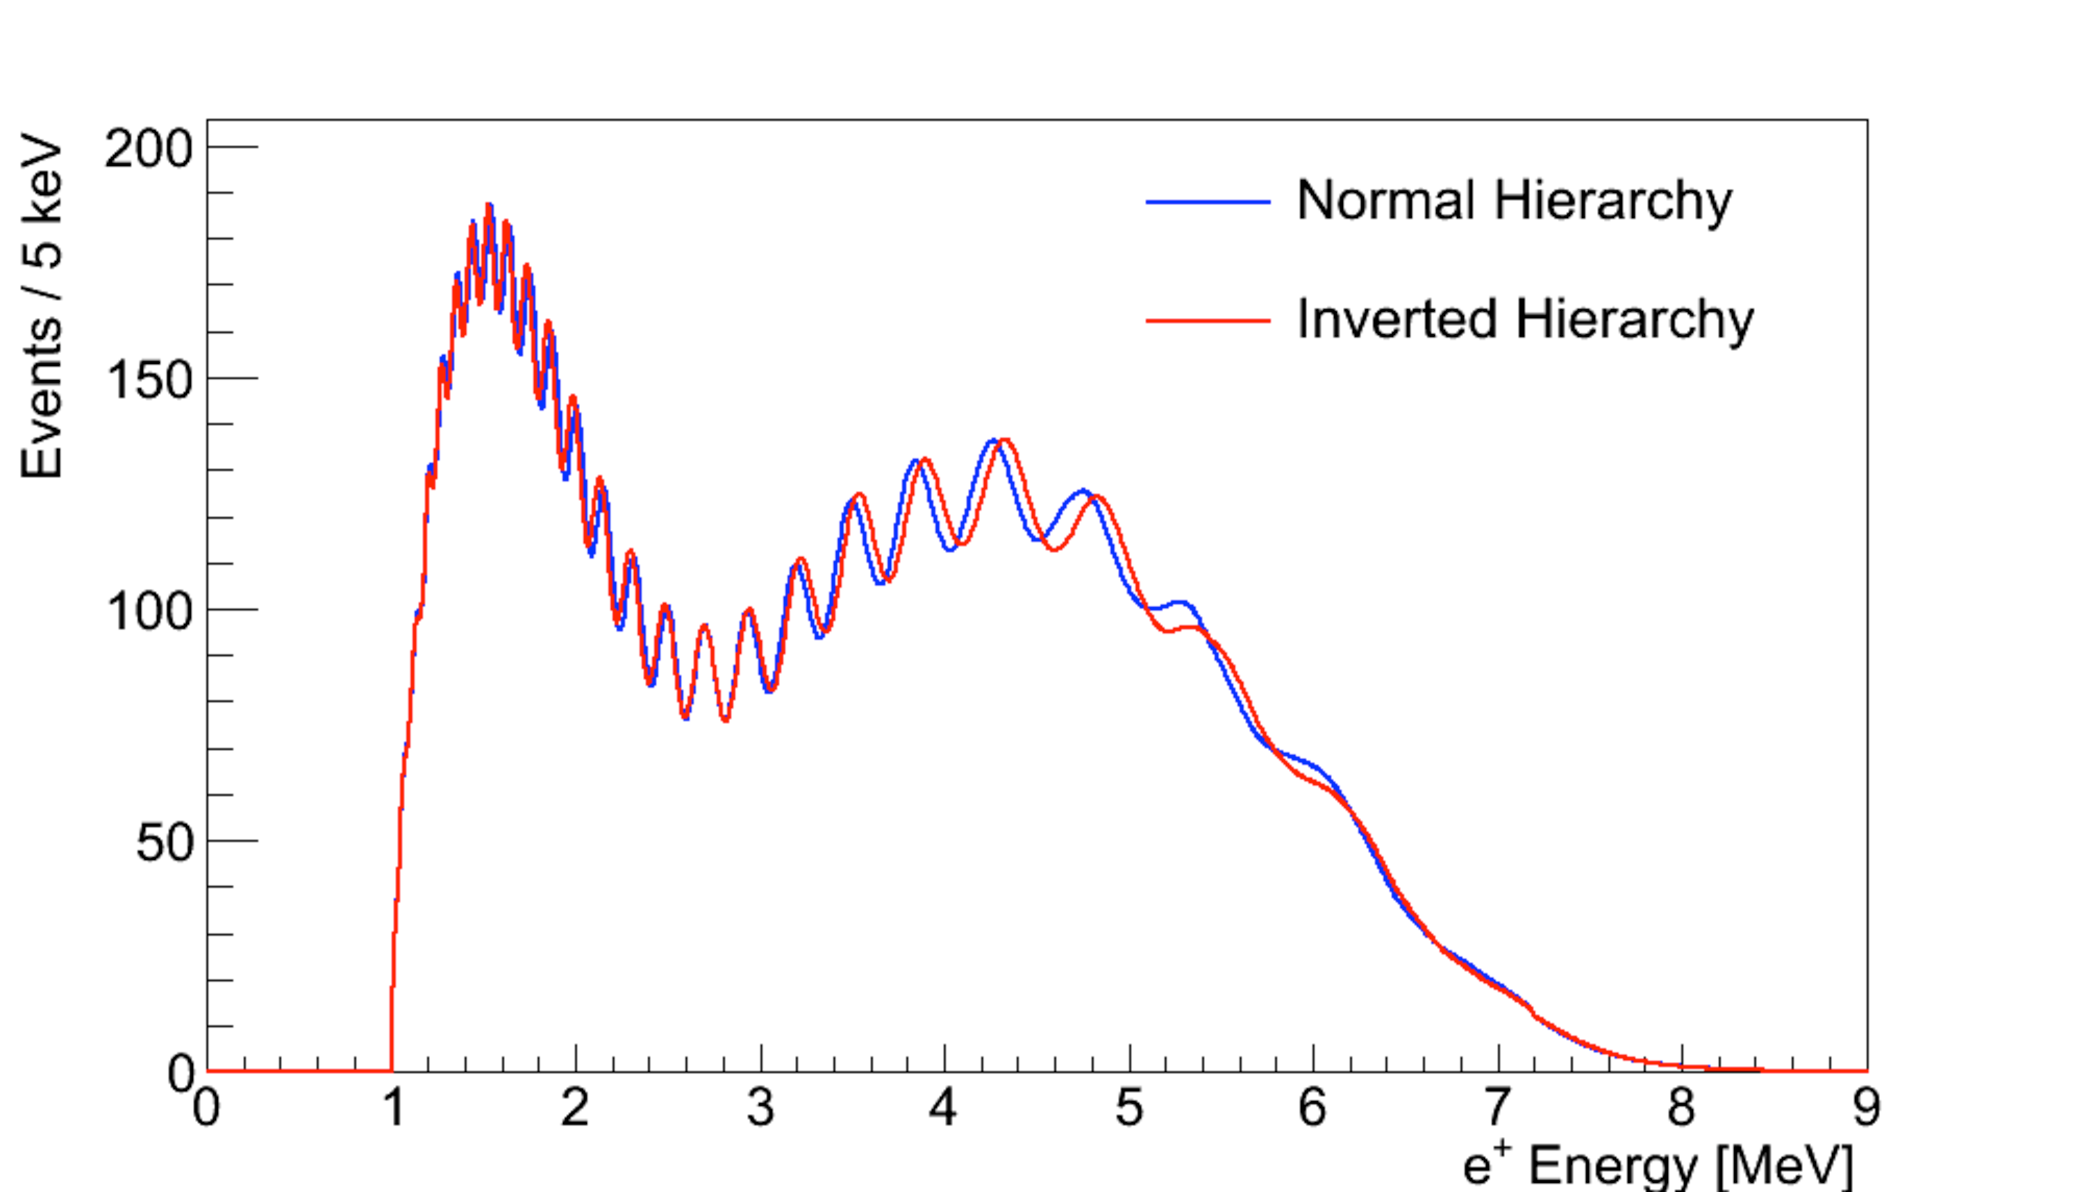
\includegraphics[width=0.7\textwidth]{DAD/worst_case_JUNO.pdf}
\caption{Estimated positron energy spectrum of the inverse-beta decay reaction for
  an ideal reactor anti-neutrino experiment (20~kton detector,
  40~GW$_{th}$ reactor power at 58~km, 5~years operation).  The solar
  oscillation (${\Delta}m^{2}_{21}$) causes the broad deficit between
  2-4~MeV.  The normal (blue) versus inverted (red) hierarchy 
results in an
  effective shift in the phase of the high-frequency oscillation.  In this example, $\Delta m^2_{31}$ has been changed to  $-\Delta m^2_{31}$ in inverting the hierarchy.}
\label{fig:reactorTrue_NoDegeneracy}
\end{figure}

JUNO is a liquid-scintillator detector very similar to KamLAND in
design, but twenty times larger in mass (20 kton)~\cite{yfwang_INPA_2013}.  It
is proposed to be built in the Jiangmen city of Guangdong province in
southern China, roughly 70 km from Macau.  The Yangjiang
(17.4~GW$_{th}$) and Taishan (18.4~GW$_{th}$) reactor facilities serve
as the electron anti-neutrino source.  The detector is located at the first
solar oscillation minimum, approximately 58~km from both reactor
facilities.

An effort based in Korea also intends to build a large scintillating
reactor anti-neutrino experiment (RENO-50). 
The original design had a marginal sensitivity to
the mass hierarchy, due to a smaller 10~kton target 
mass and poorer detector resolution than JUNO.  Recent changes to the
design goals~\cite{KimRENO} aim at a detector size of $\mathcal{O}(20)$~kton and sensitivity
similar to JUNO. RENO-50 plans to submit a Letter of Intent to funding
agencies in 2013.  

To determine the neutrino mass hierarchy, JUNO and RENO-50 will
need to improve over current standards for energy resolution and
calibration.  The JUNO collaboration's goal 
is to achieve a detector resolution of $\sigma_{E}/E$=3\%/$\sqrt{E_{e+}{\rm [MeV]}}$
in order to measure the hierarchy.  For
KamLAND, the energy resolution was limited to 6.5\%/$\sqrt{E}$ by
photoelectron statistics.  An improved resolution requires more
photons per unit of positron energy be detected.  The JUNO
experiment aims to increase photon statistics by increasing the
scintillator light yield ($\times$1.5), increasing the total
photocathode coverage ($\times$2.3), and by increasing the
efficiency of each photomultiplier ($\times$2.0) relative to those of KamLAND.
Improving the light yield and PMT efficiency have not yet been
demonstrated; both require significant technological advances.
Increasing the photocathode coverage is straightforward, only
requiring sufficient funds to purchase $\sim$15,000 20"-diameter PMTs.

The current state of the art in liquid scintillator is $\sim$2\% for gamma-ray calibration, as
demonstrated by the KamLAND experiment, although sub-percent level precision has been achieved in water Cherenkov detectors such as SNO.  
In liquid scintillator, particle-dependent scintillator quenching introduces a comparable
systematic uncertainty when estimating the positron calibration from
gamma-ray data.  The JUNO group has addressed the problem of non-linearity by fitting the actual observed energy spectrum and parameterizing the non-linearity, a process of self-calibration.

The JUNO group has produced an estimate of their sensitivity in Ref.~\cite{liyf_dyb2_2013}.  Fig.~\ref{fig:dyb2Sens} shows the
${\Delta}\chi^2$ distributions obtained for both the normal and
inverted hierarchy models as a function of ${\Delta}m^2_{ee}$.  The
degeneracy due to uncertainty in the mass-squared difference is
visible as the false minimum for the inverted hierarchy at a value of
${\Delta}m^2_{ee}$ 0.5\% from the true value.  
The collaboration finds a sensitivity to the hierarchy of more than $3\sigma$ under the assumption of a 3\%$\sqrt E$ detector energy resolution, 2\% correlated and 0.8\% uncorrelated uncertainties in reactor flux, 1\% uncertainty in the reactor flux spectrum, and 1\% uncertainty in the detector response.  This analysis takes the best-fit oscillation parameters from the most recent global analysis, and takes into account the true spatial distribution of reactor cores.  When allowing for potential future improvements in the uncertainty in $\Delta m^2_{32}$ this significance can be improved to more than $4\sigma$.  
This sensitivity has been confirmed by an independent study~\cite{reac:indep} under the same assumptions for detector performance and future precision on oscillation parameters.

\begin{figure}[tb]
\centering
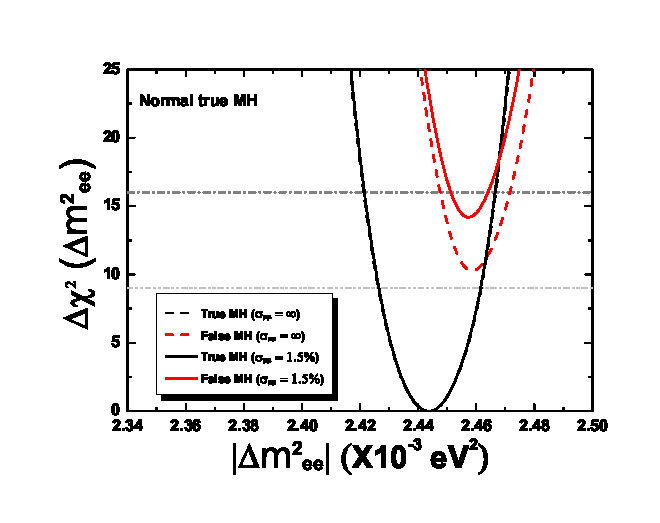
\includegraphics[width=0.7\textwidth]{DAD/Prior_NMH_15.pdf}
\caption{${\Delta}\chi^2$ distributions obtained for the normal
  (black) and inverted (red) hierarchy models as a function of
  ${\Delta}m^2_{ee}$, taken from Ref.~\cite{liyf_dyb2_2013}.  The
  degeneracy due to uncertainty in the mass-squared difference is
  visible as the false minimum for the inverted hierarchy at a value
  of ${\Delta}m^2_{ee}$ 0.5\% from the true value.  Including a
  penalty based on a 1.5\% global uncertainty in
  ${\Delta}m^2_{32}$ disfavors the inverted hierarchy at an
  additional $\sim$0.5$\sigma$ (solid red versus dashed red). }
\label{fig:dyb2Sens}
\vspace{-0.3cm}
\end{figure}

\begin{figure}[htb]
\centering
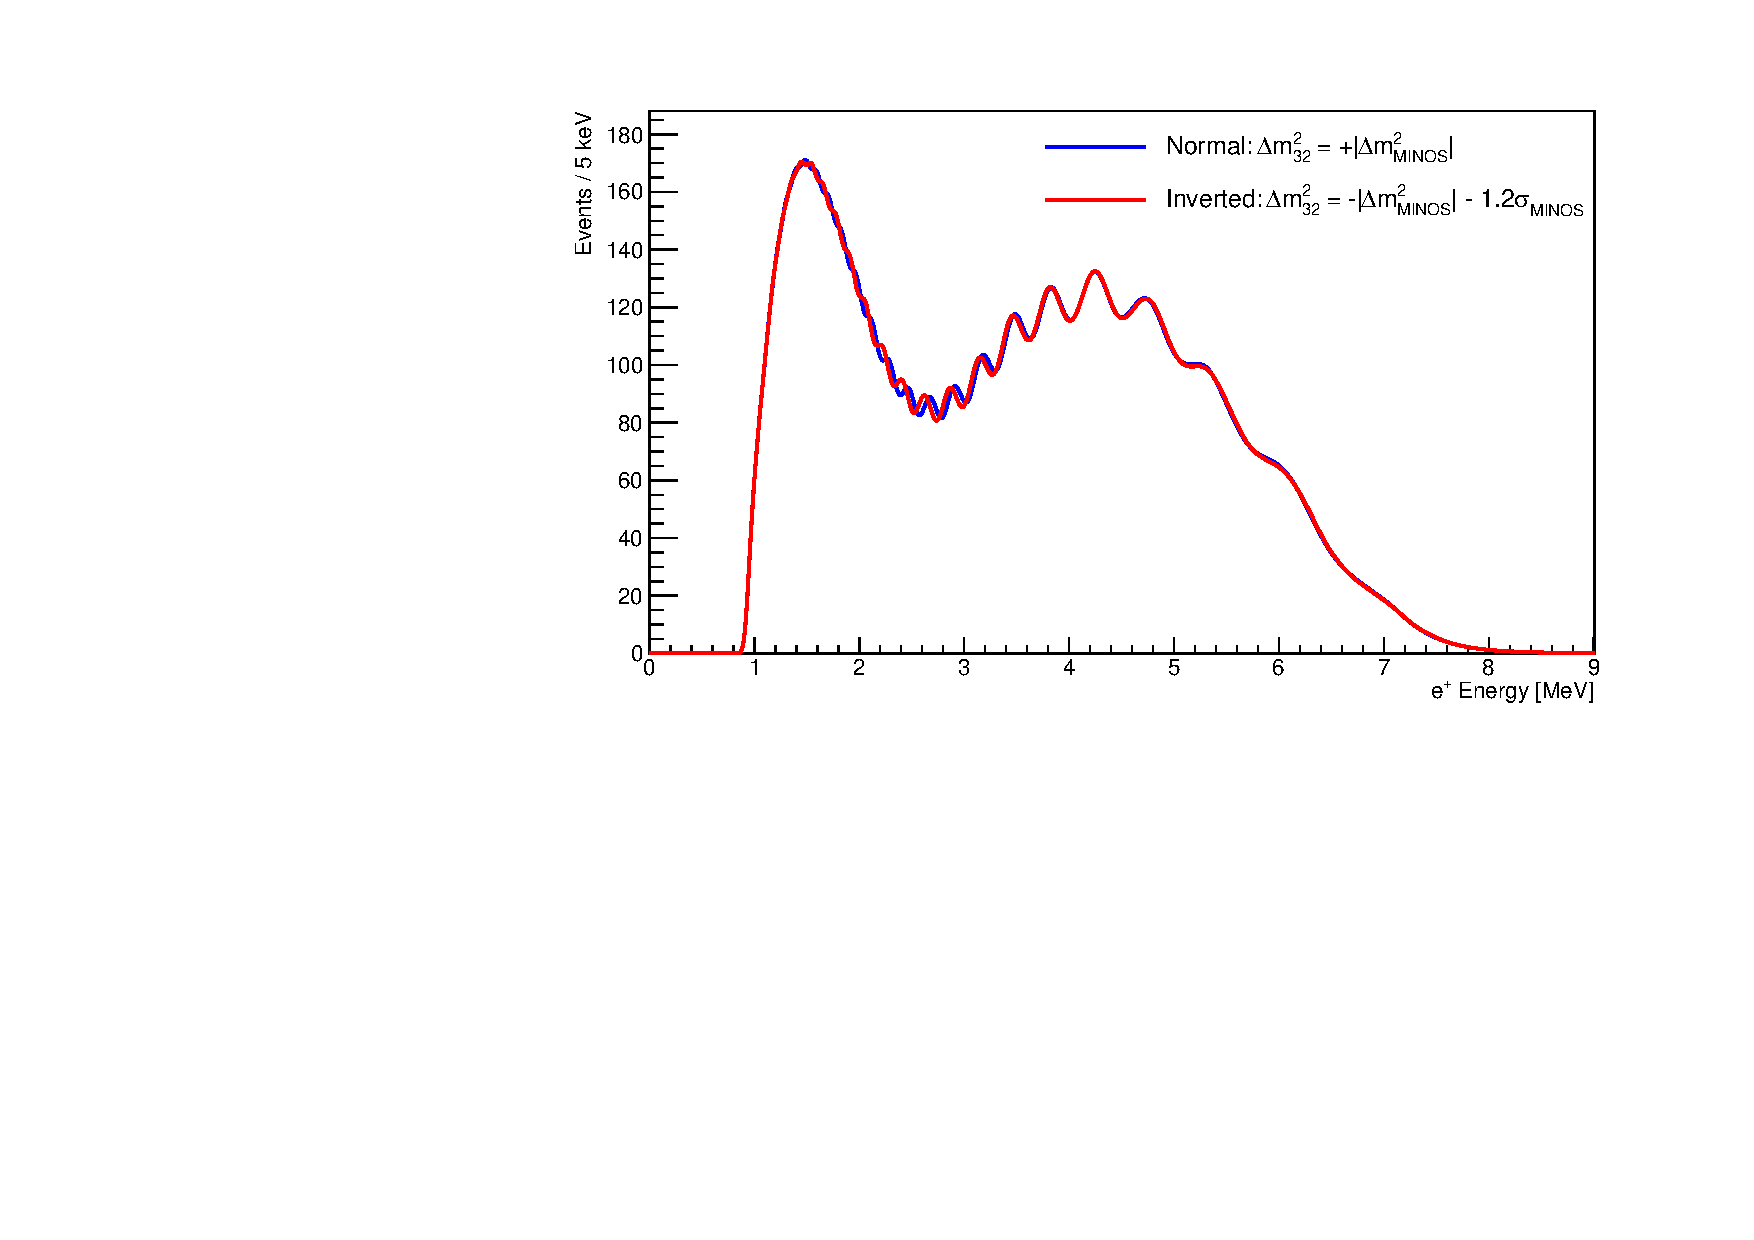
\includegraphics[width=0.7\textwidth]{DAD/positronSpectrumWithResolution_deltaMSq32.pdf}
\caption{Estimated positron energy spectrum of the inverse beta-decay reaction 
  for an ideal reactor anti-neutrino experiment (20~kton
  detector, 40~GW$_{th}$ reactor power at 58~km, 5~years operation).
  A detector energy resolution of
  $\sigma_{E}/E$=3\%/$\sqrt{E_{e+}{\rm [MeV]}}$ has been applied,
  reducing the oscillation signal below 2~MeV.  The mass difference
  for the inverted case has been shifted by 1.2$\sigma$ from the current MINOS
  best estimate (a shift of 5\%), removing the hierarchy discrimination above 3~MeV.
 }
\label{fig:reactorDet_WithDegeneracy}
\vspace{-0.3cm}
\end{figure}

The effect of finite detector resolution is to 
smear out the oscillation signal at lower positron energies.
Fig.~\ref{fig:reactorDet_WithDegeneracy} shows the expected positron
spectra, including
a detector resolution of $\sigma_{E}/E$=3\%/$\sqrt{E_{e+}{\rm [MeV]}}$ and a maximally-ambiguous 5\% shift in ${\Delta}m^2_{32}$ ($\sim 1.2\sigma$ based on the current global best fit).  The residual differences in the spectra of the
two hierarchies are limited to the 2-3~MeV region.  
Ref.~\cite{liyf_dyb2_2013} considers the effect of an improved uncertainty in ${\Delta}m^{2}_{32}$ and finds that reduction of the uncertainty to 1.5\% would result in a hierarchy significance of $3.7\sigma$, and $4.4\sigma$ if a 1\% uncertainty could be achieved.  The additional penalty to $\Delta \chi^2$ is illustrated in Fig.~\ref{fig:dyb2Sens}.


Current accelerator neutrino
experiments (T2K, NO$\nu$A) will, it is hoped, reduce the uncertainty on ${\Delta}m^{2}_{32}$ by
a factor of two.   Estimates give a global uncertainty of
1.5\% in ${\Delta}m^{2}_{32}$ by 2025.  Further reduction in this uncertainty will come from future long-baseline experiments (Section~\ref{s:lb}).



The JUNO project has an aggressive schedule~\cite{yfwang_INPA_2013}.
It has already received the Chinese equivalent of CD-1 approval.
Civil construction is targeted for 2014-2017.  Detector assembly is
planned for 2018-2019.  Data taking would commence in 2020, with a
target of 5-6~years of operation for the hierarchy measurement.

 The main challenges for JUNO are technological.  To obtain
sufficient detector resolution requires multiple factors of two
improvements in detector technology: improved scintillator light yield,
attenuation length, and PMT efficiency.  Constraints on detector
uniformity and linearity are demanding, and will likely require the
development of new methods to calibrate the detector response to
positrons.   These challenges must be met successfully if the subtle effect of the neutrino mass hierarchy on the observed positron signal is to tell us whether the neutrino mass hierarchy is normal or inverted.


















